\clearpage
\appendix
\counterwithin{equation}{section}
\renewcommand{\theequation}{\thesection.\arabic{equation}}

\section{证明}
\label{app:proofs}

\subsection{后代与报告模型}
\label{app:model}

成功次数为 $r$、成功概率为 $p$ 的负二项分布 $\NB(r,p)$ 的均值为 $r(1-p)/p$，方差为 $r(1-p)/p^2$。令 $r=k$、$p=k/(k+R_t)$，即得式~(\ref{eq:offspring})。$n$ 个相互独立的 $\NB(k,p)$ 变量之和服从 $\NB(nk,p)$；以保留概率 $\rho$ 对 $\NB(r,k/(k+\mu))$ 作二项稀疏化，得到 $\NB(r,k/(k+\rho\mu))$。结合这两条性质即得式~(\ref{eq:observed})。

\subsection{当期目标量}
\label{app:target1}

记 $C_t$ 的观测值为 $c$。由式~(\ref{eq:observed})，给定 $n$ 时 $R_t$ 的对数似然为：
\begin{equation}
  \ell(R_t)=\text{const}+nk\log\frac{k}{k+\rho R_t}+c\log\frac{\rho R_t}{k+\rho R_t},
\end{equation}
相应的得分函数可写为：
\begin{equation}
  \dot{\ell}(R_t)=\frac{c}{R_t}-\frac{(c+nk)\rho}{k+\rho R_t}=\mathcal{I}(R_t)\,(\Rhat_t-R_t),\qquad % qa-allow: display-math separator kept verbatim from EN
  \mathcal{I}(R_t)=\frac{n}{R_t/\rho+R_t{}^2/k},
  \label{eq:score}
\end{equation}
其中 $\mathcal{I}(R_t)$ 为 Fisher 信息。$\Rhat_t=c/(\rho n)$ 的条件均值为 $R_t$，条件方差为 $R_t/(\rho n)+R_t{}^2/(kn)=1/\mathcal{I}(R_t)$。由于得分函数与 $\Rhat_t-R_t$ 成正比，对任意有限的 $n$，Cram\'er--Rao 下界均可达到。式~(\ref{eq:observed}) 中的分布是关于 $C_t$ 的单参数指数族，其自然参数 $\log[\rho R_t/(k+\rho R_t)]$ 的取值范围为一个开区间，因此 $C_t$ 为完备充分统计量，$\Rhat_t$ 为 $R_t$ 的一致最小方差无偏估计量\citep{lehmann2005testing}。

\subsection{命题~\ref{prop:average} 的证明}
\label{app:prop1}

在假设 H4 下，$\E(R_t\mid n)=\Rbar$，$\Var(R_t\mid n)=v_R$。由全方差公式与附录~\ref{app:target1} 的结果，误差方差为：
\begin{equation}
  \Var(\Rhat_t\mid n)=\E\!\left[\frac{R_t}{\rho n}+\frac{R_t{}^2}{kn}\right]+\Var(R_t)=v_R+\frac{\Rbar}{\rho n}+\frac{\Rbar^2+v_R}{kn},
\end{equation}
代入 $m=\rho n$ 即得式~(\ref{eq:var-average})。结论（i）与（ii）由取极限得到。对于结论（iii），$[V(m)-V(2m)]/V(m)=[A/(2m)]/(v_R+A/m)=1/[2(1+m/\mx)]$，在 $m=\mx$ 处等于四分之一。对于结论（iv），设 $\tilde{\theta}$ 为基于第 $t$ 期数据且满足 $\E(\tilde{\theta}\mid R_t)=R_t$ 的任一估计量，则 $\E(\tilde{\theta}-\Rbar)^2=\E[\Var(\tilde{\theta}\mid R_t)]+v_R\ge\E[1/\mathcal{I}(R_t)]+v_R=V$，取 $\Rhat_t$ 时等号成立。当 $R_{t+1}$ 与历史独立时，对 $y=C_{t+1}/m$ 作一步预测，有 $\E(\hat{y}-y)^2=(\hat{y}-\E y)^2+\Var(y)\ge V$，且在 $\hat{y}=\Rbar$ 处取等号。

覆盖规模与报告完整度的边际效应分别为 $-\partial V/\partial\log n=A/m$ 和 $-\partial V/\partial\log\rho=\Rbar/m$，二者之比为 $A/\Rbar$。若 $R_t$ 为平稳一阶自回归过程，其方差为 $v_R$，相邻时期的相关系数为 $\phi$，则给定 $R_t$ 时 $R_{t+1}$ 的最优线性预测的误差方差为 $(1-\phi^2)v_R$\citep{hamilton1994time}。对于方差同为 $v_R$、平均两两相关系数为 $\bar{c}$ 的 $J$ 个辖区，其均值的方差为 $J^{-2}[Jv_R+J(J-1)\bar{c}v_R]$，由此得到式~(\ref{eq:pooling})。

\subsection{命题~\ref{prop:report-noise} 的证明}
\label{app:prop2}

记 $\sigma^2=\Var(p_t)=\tau^2\rho^2$。给定 $(n,R_t,p_t)$ 时，$C_t$ 的均值为 $p_tnR_t$，方差为 $p_tnR_t+p_t{}^2nR_t{}^2/k$。对 $p_t$ 取平均，给定 $(n,R_t)$ 的条件方差为：
\begin{equation}
  \Var(C_t\mid n,R_t)=\rho nR_t+\frac{(\rho^2+\sigma^2)nR_t{}^2}{k}+\sigma^2n^2R_t{}^2.
\end{equation}
条件均值为 $\rho nR_t$，因此 $\Rhat_t$ 仍是 $\Rbar$ 的无偏估计量。再对 $R_t$ 取平均并除以 $(\rho n)^2$，得：
\begin{equation}
  V_H(m)=v_R+\tau^2(\Rbar^2+v_R)+\frac{\Rbar}{m}+\frac{\rho(1+\tau^2)(\Rbar^2+v_R)}{km},
\end{equation}
此即式~(\ref{eq:vH-AH})。记 $U=(1+\tau^2)(\Rbar{}^2+v_R)$，则极限误差方差为 $v_R+v_H=U-\Rbar{}^2$，且 $A_H=\Rbar+\rho U/k$，因此 $\Rhat_t$ 的均值与方差仅通过 $U$ 依赖于 $v_R$ 与 $\tau$。不等式 $m_{\times,H}<\mx$ 等价于 $\rho v_R/k<A$；由于 $\Rbar^2+v_R>v_R$，后一不等式成立。

\subsection{命题~\ref{prop:allocation} 的证明}
\label{app:prop3}

给定 $(R_1,\dots,R_T)$ 时，不同时期的病例数相互独立。记 $\bar{R}_T=T^{-1}\sum_tR_t$，则均值估计的方差为：
\begin{equation}
  \Var\!\Big(\frac{1}{T}\sum_{t=1}^T\Rhat_t\Big)=\Var(\bar{R}_T)+\frac{A}{Tm},
\end{equation}
其中各期独立时 $\Var(\bar{R}_T)=v_R/T$，由此得到式~(\ref{eq:alloc-indep})。对于满足 $\Cov(R_s,R_t)=v_R\phi^{|s-t|}$ 的平稳一阶自回归过程，有 $T^2\Var(\bar{R}_T)=v_R[T+2\sum_{h=1}^{T-1}(T-h)\phi^h]$，对几何级数求和即得式~(\ref{eq:ar-sum})\citep{hamilton1994time}。将 $T=\mathcal{B}/(c_0+c_1m)$ 代入式~(\ref{eq:alloc-indep})，得到目标函数：
\begin{equation}
  f(m)=\frac{(c_0+c_1m)(v_R+A/m)}{\mathcal{B}}=\frac{c_0v_R+c_1A+c_1v_Rm+c_0A/m}{\mathcal{B}},
\end{equation}
当 $c_0>0$ 时 $f(m)$ 严格凸，且 $f'(m)=(c_1v_R-c_0A/m^2)/\mathcal{B}$。唯一驻点满足 $m^{*2}=c_0A/(c_1v_R)=(c_0/c_1)\mx$，即式~(\ref{eq:optimal-m})。

\subsection{推论~\ref{cor:switch} 的证明}
\label{app:cor1}

记 $U_0=\Rbar^2+v_R$。由式~(\ref{eq:vH-AH})，按比例提高覆盖规模与报告完整度所带来的收益分别为：
\begin{equation}
  -\frac{\partial V_H}{\partial\log n}=\frac{\Rbar}{\rho n}+\frac{(1+\tau^2)U_0}{kn},\qquad % qa-allow: display-math separator kept verbatim from EN
  -\frac{\partial V_H}{\partial\log\rho}=\frac{\Rbar}{\rho n}-\rho\frac{\mathrm{d}\tau^2}{\mathrm{d}\rho}\,U_0\left(1+\frac{1}{kn}\right).
\end{equation}
若 $\mathrm{d}\tau^2/\mathrm{d}\rho=0$，第一项收益比第二项收益大 $(1+\tau^2)U_0/(kn)>0$。对 $\nu$ 个单位作二项抽样时，有 $\tau^2=(1-\rho)/[\rho(\nu+1)]$ 及 $\rho\,\mathrm{d}\tau^2/\mathrm{d}\rho=-1/[\rho(\nu+1)]$。此时第二项收益减去第一项收益的差为：
\begin{equation}
  \frac{U_0}{kn}\left[\frac{kn+\rho}{\rho(\nu+1)}-1\right],
\end{equation}
该差值当且仅当 $kn>\rho\nu$，即 $m>\rho^2\nu/k$ 时为正。

\subsection{更新方程表述与分母噪声}
\label{app:renewal}

令 $\bar{\Lambda}=\E(\Lambda_{t+1}\mid\mathcal{F}_t)$，$m=\rho\bar{\Lambda}$。以 $(\Lambda_{t+1},R_{t+1})$ 为条件并应用全方差公式，预测方差为：
\begin{equation}
  \Var(C_{t+1}\mid\mathcal{F}_t)=mA+\rho^2\bar{\Lambda}^2\left[v_R+\mathrm{CV}^2(\Lambda_{t+1}\mid\mathcal{F}_t)\,(\Rbar^2+v_R)\right],
\end{equation}
除以 $m^2$ 即得式~(\ref{eq:info-decomp})。对于式~(\ref{eq:b-delta})，记 $D_t=m(1+\delta)$，其中 $\E\delta=0$，$\E\delta^2=c_w/m$，$c_w=(1-\rho)\sum_sw_s{}^2$；并令 $Y=C_{t+1}/m$ 与 $\delta$ 独立，其均值为 $\Rbar$，方差为 $v_R+A/m$。将 $G_t=Y(1+\delta)^{-1}$ 展开到二阶，得：
\begin{equation}
  \E(G_t)=\Rbar\left(1+\frac{c_w}{m}\right)+O(m^{-2}),\qquad % qa-allow: display-math separator kept verbatim from EN
  \Var(G_t)=v_R+\frac{A+(\Rbar^2+3v_R)c_w}{m}+O(m^{-2}),
\end{equation}
再除以 $[\E(G_t)]^2=\Rbar^2(1+2c_w/m)+O(m^{-2})$。精确到 $1/m$ 一阶项时，相对方差为 $v_R/\Rbar^2+[A+(\Rbar^2+v_R)c_w]/(\Rbar^2m)$，此即式~(\ref{eq:b-delta})。

\section{扩展}
\label{app:extensions}

\subsection{环境方差的估计精度}
\label{app:vr-precision}

\begin{proposition}[环境方差的估计精度]
\label{prop:vr-precision}
设 $R_1,\dots,R_T$ 为相互独立的伽马变量，其均值 $\Rbar$ 已知、方差为 $v_R$，并令 $\xi=\Rbar^2/v_R$。基于 $T$ 个时期病例数的任一 $v_R$ 无偏估计量，其相对标准误的下界为：
\begin{equation}
  \left[T\xi\left(\xi\psi'(\xi)-1\right)\right]^{-1/2},
  \label{eq:vr-bound}
\end{equation}
其中 $\psi'$ 为三伽马函数。当 $\xi\to\infty$ 时，此下界趋于高斯情形下的值 $\sqrt{2/T}$。
\end{proposition}

\begin{proof}[证明]
病例数仅通过 $R_{1:T}$ 依赖于 $v_R$，因此由数据处理不等式，病例数所含关于 $v_R$ 的 Fisher 信息不超过 $R_{1:T}$ 所含的相应信息。固定均值时，伽马分布的形状参数为 $\xi$，尺度参数为 $v_R/\Rbar$。单个观测所含关于 $\xi$ 的信息为 $\psi'(\xi)-1/\xi$，且 $\mathrm{d}\xi/\mathrm{d}v_R=-\xi/v_R$，因此 $T$ 个时期所含关于 $v_R$ 的信息为 $T\xi(\xi\psi'(\xi)-1)/v_R{}^2$。由 Cram\'er--Rao 不等式即得式~(\ref{eq:vr-bound})。极限结论由 $\psi'(\xi)=1/\xi+1/(2\xi^2)+O(\xi^{-3})$ 得到。
\end{proof}

在表~\ref{tab:s7} 的基线设定（$\Rbar=1.15$，$v_R=0.04$）下，$\xi=33.06$，$\xi(\xi\psi'(\xi)-1)=0.505$，因此相对标准误在 3 个时期时至少为 0.812，在 10 个时期时至少为 0.445，在 50 个时期时至少为 0.199。常数 0.505 仅对应这一基线，式~(\ref{eq:vr-bound}) 给出一般形式。

\subsection{自相关环境下的预算阈值}
\label{app:budget-ar}

存在自相关 $\phi$ 时，命题~\ref{prop:allocation} 中的环境项为 $v_Re(T)$，其中 $e(T)=S(\phi,T)/T^2$。将 $T$ 视为连续变量，定义 $g_T=-T^2e'(T)$，于是各期独立时 $g_T=1$；再令 $m_0{}^*=\sqrt{(c_0/c_1)\mx}$ 为式~(\ref{eq:optimal-m}) 给出的最优值。

\begin{proposition}[预算阈值]
\label{prop:budget-ar}
在预算约束 $\mathcal{B}=T(c_0+c_1m)$ 下，每期最优病例量满足 $m^*=m_0{}^*(g_{T^*})^{-1/2}$，其中 $T^*$ 为最优时期数。若 $g_T$ 随 $T$ 递增，由 $g_1<1$ 趋向 $(1+\phi)/(1-\phi)>1$，则存在唯一的 $T^\dagger$ 使 $g_{T^\dagger}=1$；当 $T^*<T^\dagger$ 时 $m^*$ 大于 $m_0{}^*$，当 $T^*>T^\dagger$ 时则小于这一取值。两种情形在如下预算处衔接：
\begin{equation}
  \mathcal{B}^\dagger=T^\dagger\left(c_0+c_1m_0{}^*\right),
  \label{eq:b-dagger}
\end{equation}
当 $c_1=1$ 时，$\mathcal{B}^\dagger$ 以每个报告病例的成本为单位。
\end{proposition}

\begin{proof}[证明]
将抽样项写为 $Ac_1/(\mathcal{B}-c_0T)$，并将 $v_Re(T)+Ac_1/(\mathcal{B}-c_0T)$ 对 $T$ 求导，得一阶条件 $v_Rg_T=c_0A/(c_1m^2)$，因此 $m^{*2}=m_0{}^{*2}/g_{T^*}$。$m^*$ 与 $m_0{}^*$ 的大小关系由 $g_T$ 的单调性得到；当 $T^*=T^\dagger$ 时，由预算约束即得式~(\ref{eq:b-dagger})。
\end{proof}

当 $\phi=0.8$ 时，$g_T$ 随 $T$ 递增，且 $T^\dagger=4.484$。取 $c_0/c_1=100$ 并采用基线平衡规模，得 $m_0{}^*=72.86$，$\mathcal{B}^\dagger=775.0$；在第~\ref{sec:meth-loss}~节所用的 21.3--49.2 例潜伏平衡规模范围内，$\mathcal{B}^\dagger$ 的取值范围为 655.3--762.8（表~\ref{tab:s7}）。上述计算将 $T$ 视为连续变量，并假定环境过程平稳，因此适用于单个流行季内部，不适用于平均传播强度不同的多个流行季之间。

\subsection{流行季间方差}
\label{app:seasons}

\begin{corollary}[流行季层面的下界]
\label{cor:season}
设流行季效应 $\eta_1,\dots,\eta_S$ 为相互独立的高斯变量，其均值未知、方差为 $v_S$，且病例数仅通过流行季效应依赖于 $v_S$。基于病例数的任一 $v_S$ 无偏估计量，其相对标准误不小于 $\sqrt{2/(S-1)}$；$S=3$ 时此下界为 1.00，$S=4$ 时为 0.816。
\end{corollary}

\begin{proof}[证明]
设 $\delta$ 为基于病例数的无偏估计量。由于给定 $\eta_{1:S}$ 时病例数的条件分布不依赖于 $v_S$，$\E(\delta\mid\eta_{1:S})$ 是流行季效应的函数且对 $v_S$ 无偏，其方差不超过 $\delta$ 的方差。$\eta_{1:S}$ 的样本均值与样本方差构成完备充分统计量，因此样本方差是 $v_S$ 的最小方差无偏估计量，其方差为 $2v_S{}^2/(S-1)$\citep{lehmann2005testing, searle1992variance}。
\end{proof}

由于跨流行季的均值需要估计，上述下界使用 $S-1$ 个自由度；均值已知时的相应下界 $\sqrt{2/S}$ 更小（表~\ref{tab:s7}）。三个和四个流行季的季别截距另列于表~\ref{tab:s5}。

\subsection{检验传播是否超过 1}
\label{app:ump}

当 $R>R'$ 时，由于 $R/(k+\rho R)$ 随 $R$ 递增，式~(\ref{eq:observed}) 的似然比随 $c$ 递增，因此这一分布族关于 $C_t$ 具有单调似然比。于是，当 $C_t\ge c_\alpha$ 时拒绝 $R_t\le1$ 的检验，其功效函数随 $R_t$ 不减；由 Karlin--Rubin 定理，此检验在实际达到的水平 $\alpha^*=P_{R_t=1}(C_t\ge c_\alpha)\le\alpha$ 上为一致最优势检验\citep{karlin1956theory, lehmann2005testing}。由于 $C_t$ 为离散变量，$\alpha^*$ 一般低于名义水平；除非采用随机化检验或使用 mid-$p$ 值，最优性仅在 $\alpha^*$ 处成立，在 $\alpha$ 处不成立。

\subsection{收缩估计给出的理想下界}
\label{app:shrinkage}

命题~\ref{prop:average} 的结论（iv）排除了在给定 $R_t$ 时有偏的估计量。考虑 $\hat{\theta}_\lambda=(1-\lambda)\Rhat_t+\lambda\mu_0$，其中 $\mu_0$ 为固定基准，$\Delta=\mu_0-\Rbar$。$\hat{\theta}_\lambda$ 作为 $\Rbar$ 的估计，其均方误差为：
\begin{equation}
  \mathrm{MSE}(\lambda)=(1-\lambda)^2V+\lambda^2\Delta^2,
\end{equation}
其中 $V$ 由式~(\ref{eq:var-average}) 给出。最小值在 $\lambda^*=V/(V+\Delta^2)$ 处取得，此时 $\mathrm{MSE}(\lambda^*)=V\Delta^2/(V+\Delta^2)$；当且仅当 $\Delta^2<v_R(1+m/\mx)$ 时，这一最小值低于 $v_R$。权重 $\lambda^*$ 依赖未知的 $\Rbar$ 与 $V$，因此上述结果只构成理想下界，无法作为可行估计量使用；经验贝叶斯估计量或分层估计量从数据中估计权重，无法达到这一下界\citep{stoner2019hierarchical}。

\clearpage
\section{补充图}
\label{app:figure}

\begin{figure}[htbp]
  \centering
  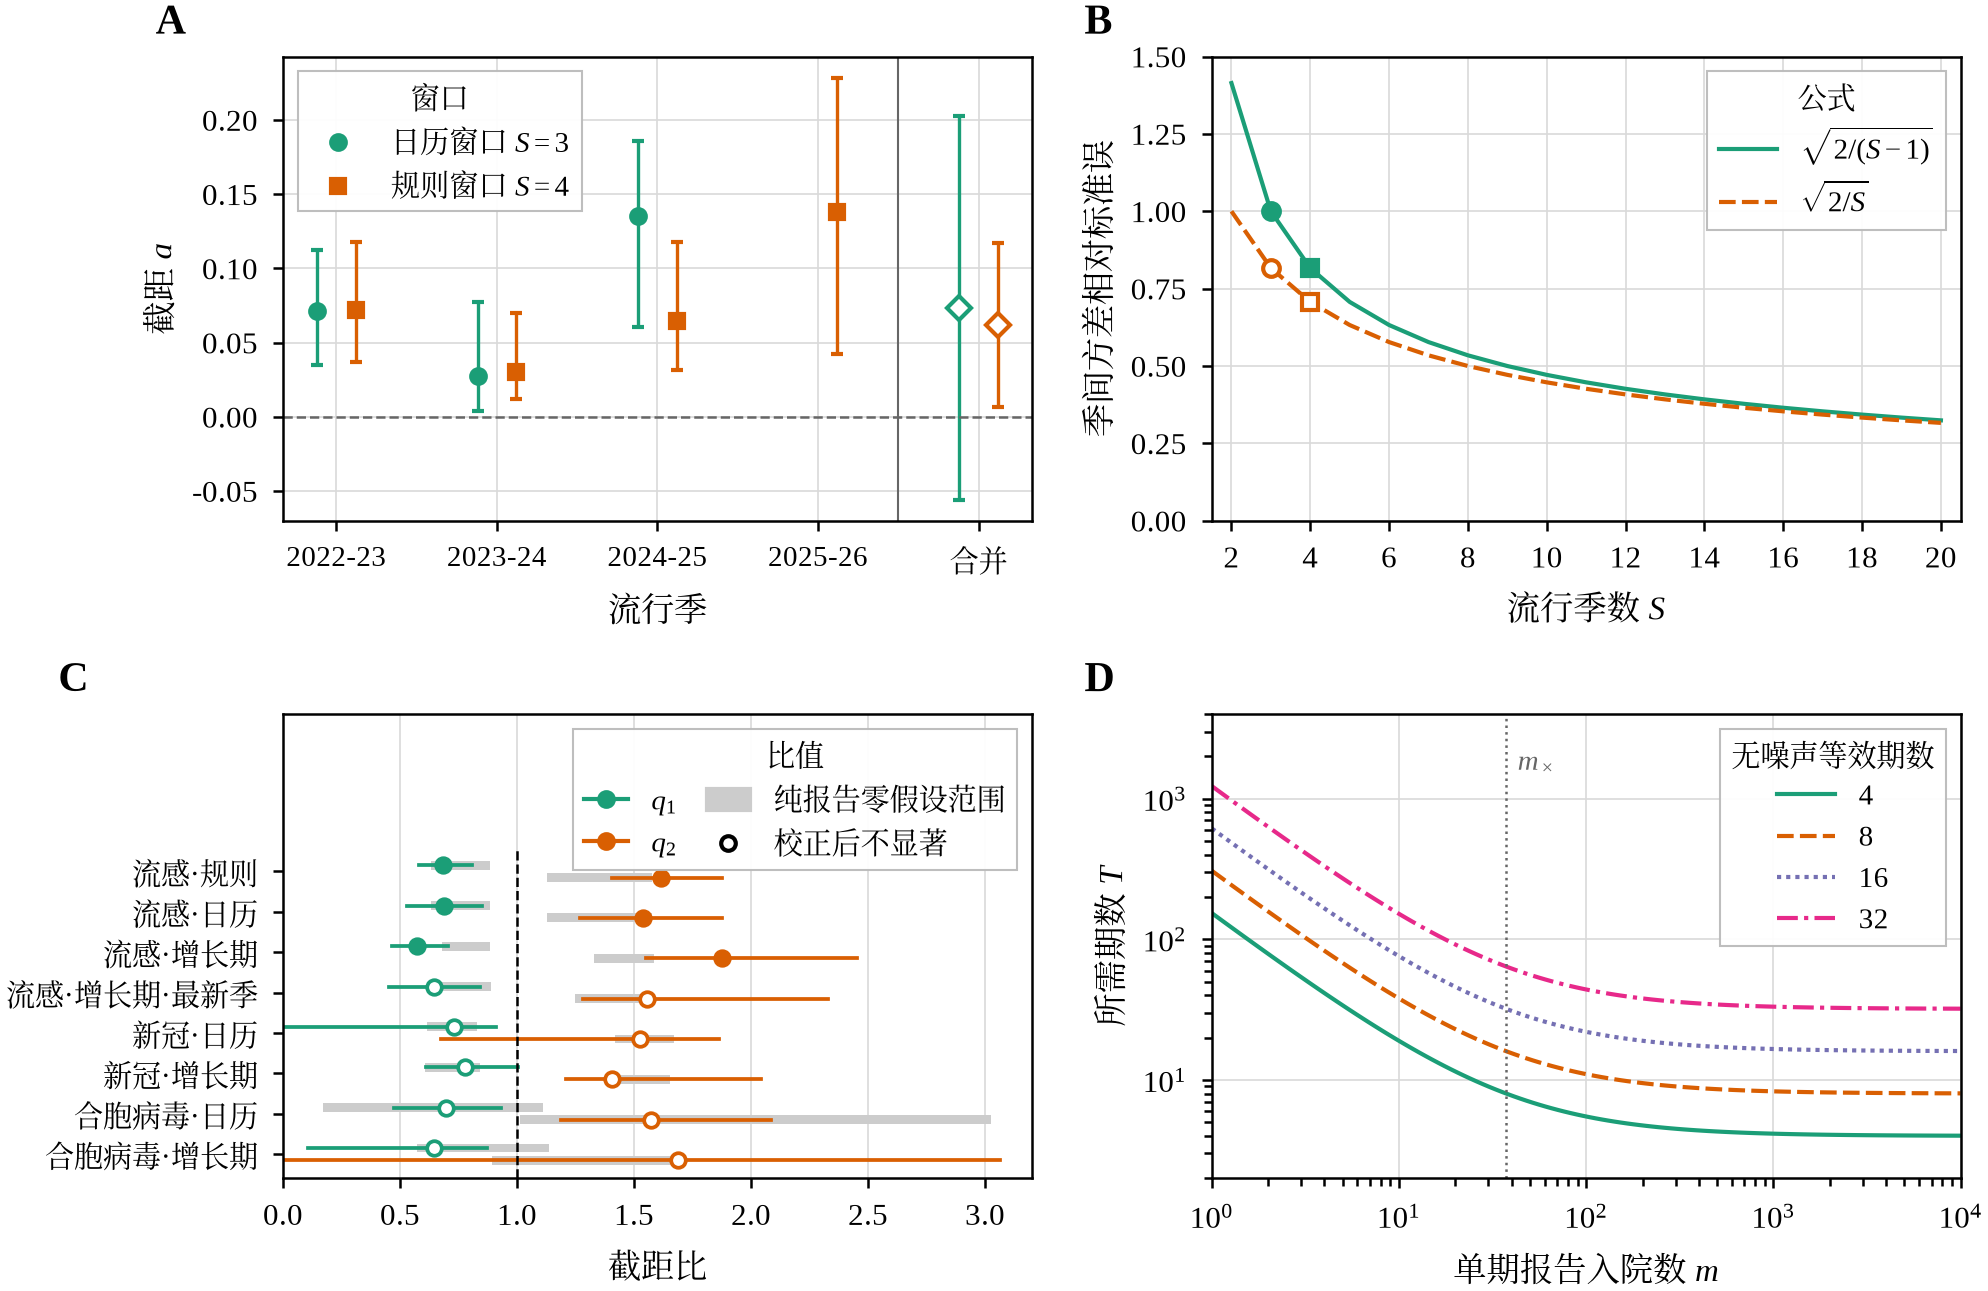
\includegraphics[width=0.86\linewidth]{figures/fig_07_seasons_pathogens_design.png}
  \caption{季间不确定性、不同病原体的截距比与所需时期数。（A）加权增长比在日历窗口和按规则界定的早期增长窗口中的分季截距，误差线为双向自助法 95\% 区间；空心菱形为随机效应合并估计。（B）季间方差估计的相对标准误下界随流行季数的变化，并与先前分析报告的数值比较。（C）单周分母与三周等权分母相对于原始权重的截距比；灰条为无环境变异时仅由报告噪声和流行增长所预期的范围，实心标记表示经 Holm 校正后仍显著的单侧检验。（D）不同单期报告住院人数下，达到给定数量无噪声时期的精度所需的时期数；本面板仅作示意，已由图~\ref{fig:design}A 的实证列线图取代。}
  \label{fig:seasons}
\end{figure}

\FloatBarrier
\clearpage
\section{补充表格}
\label{app:tables}

\setcounter{table}{0}
\renewcommand{\thetable}{S\arabic{table}}

表~\ref{tab:s1}--\ref{tab:s7} 报告图~\ref{fig:floor}--\ref{fig:seasons} 所依据的估计值。表~\ref{tab:s4} 将自愿报告期与强制报告年份中相同日历月份的数据进行比较。表~\ref{tab:s8} 给出反演在各设定下的隐含环境方差（图~\ref{fig:inversion}），表~\ref{tab:s9} 列出本分析各轮所用的设定。全部数值均由分析代码保存的输出生成。

\begin{table}[htbp]
\centering
\footnotesize
\caption{各设定下相对损失的截距 $a$、斜率 $b$ 与平衡比 $b/a$，以及各估计值的双向自助法 95\% 置信区间。}
\label{tab:s1}
\begin{tabular}{lrrrlllr}
\toprule
设定 & $N$ & 周数 & $\bar{x}$ & $a$ [95\% CI] & $b$ [95\% CI] & $b/a$ [95\% CI] & 标准差比 \\
\midrule
$R_A$，规则窗口（$S=4$） & 1748 & 42 & 1.206 & 0.0150 [0.0100, 0.0208] & 0.560 [0.367, 0.769] & 37.4 [19.1, 71.0] & 1.95 \\
$G$，规则窗口（$S=4$） & 1756 & 42 & 1.724 & 0.0840 [0.0498, 0.1248] & 1.971 [0.959, 3.098] & 23.5 [8.4, 59.7] & 2.29 \\
$G$，日历窗口（$S=3$） & 1267 & 29 & 1.671 & 0.0991 [0.0569, 0.1382] & 2.243 [1.060, 3.559] & 22.6 [9.0, 52.2] & 4.68 \\
$R_A$，日历窗口（$S=3$） & 1263 & 29 & 1.190 & 0.0202 [0.0097, 0.0306] & 0.516 [0.279, 0.839] & 25.6 [10.2, 79.6] & 3.46 \\
\bottomrule
\end{tabular}
\par\smallskip
\begin{minipage}{0.95\linewidth}\scriptsize 以迭代 FGLS 将 $L=((x-\bar{x})/\bar{x})^2$ 拟合为 $a+b/D$；区间为州 $\times$ 周双向鸽笼自助法 95\% 百分位区间，$B=2000$，每次重抽重新估计 $\bar{x}$。标准差比为双向重抽与仅按州重抽下 $a$ 的自助标准差之比。均为 51 个辖区。\end{minipage}
\end{table}

\begin{table}[htbp]
\centering
\footnotesize
\caption{截距分解及仿射模型与幂律的比较，附各截距的 95\% 置信区间。}
\label{tab:s2}
\setlength{\tabcolsep}{4pt}
\begin{tabular}{lllrrrrrr}
\toprule
设定 & $a$ 总量 & \begin{tabular}[t]{@{}c@{}}去除周效应\\ 后的 $a$\end{tabular} & \begin{tabular}[t]{@{}c@{}}去除周效应与州-季\\ 效应后的 $a$\end{tabular} & 周占比 & ICC & 幂指数 & $p$ & \begin{tabular}[t]{@{}c@{}}交叉验证折数\\（州；季）\end{tabular} \\
\midrule
$R_A$，规则窗口（$S=4$） & \begin{tabular}[t]{@{}c@{}}0.0150\\ \relax[0.0100, 0.0208]\end{tabular} & \begin{tabular}[t]{@{}c@{}}0.0088\\ \relax[0.0064, 0.0124]\end{tabular} & \begin{tabular}[t]{@{}c@{}}0.0083\\ \relax[0.0064, 0.0141]\end{tabular} & 0.41 & 0.25 & 0.38 & 0.11 & 26/51；2/4 \\
$G$，规则窗口（$S=4$） & \begin{tabular}[t]{@{}c@{}}0.0840\\ \relax[0.0508, 0.1226]\end{tabular} & \begin{tabular}[t]{@{}c@{}}0.0415\\ \relax[0.0306, 0.0586]\end{tabular} & \begin{tabular}[t]{@{}c@{}}0.0394\\ \relax[0.0293, 0.0614]\end{tabular} & 0.51 & 0.31 & 0.35 & 0.44 & 19/51；0/4 \\
$G$，日历窗口（$S=3$） & \begin{tabular}[t]{@{}c@{}}0.0991\\ \relax[0.0583, 0.1399]\end{tabular} & \begin{tabular}[t]{@{}c@{}}0.0473\\ \relax[0.0337, 0.0676]\end{tabular} & \begin{tabular}[t]{@{}c@{}}0.0450\\ \relax[0.0335, 0.0932]\end{tabular} & 0.52 & 0.29 & 0.27 & 0.42 & 28/51；3/3 \\
\bottomrule
\end{tabular}
\par\smallskip
\begin{minipage}{0.95\linewidth}\scriptsize 区间来自 $B=1000$ 的双向自助法，其抽样与表 S1 相互独立，因此数值略有差异。第三列在拟合前从统计量中去除全国周效应，第四列再去除州-季效应。周占比等于一减去第三列与第二列之比。ICC 为统计量方差中位于周间的份额。幂指数为 $L=\alpha D^{-c}$ 中的 $c$；$p$ 来自仿射模型对该幂律的参数自助检验，零分布抽样 200 次。交叉验证折数为逐州留一与逐季留一时仿射模型预测更优的折数。功效分析表明，真实截距取估计 $a$ 的任何比例（$\le 1$）时，检验功效均达不到 80\%。\end{minipage}
\end{table}

\begin{table}[htbp]
\centering
\footnotesize
\caption{医院报告完整度对截距贡献的等效性检验，以及各变化量的配对自助法 90\% 置信区间。}
\label{tab:s3}
\begin{tabular}{llrlrlr}
\toprule
设定 & $10^3\Delta a$ [90\% CI] & $10^3\delta_{0.10}$ & 等效 & $10^3\delta_{0.05}$ & 等效 & 等效季数 \\
\midrule
$R_A$，规则窗口（$S=4$） & 0.29 [$-$0.22, 0.85] & 2.55 & 是 & 0.64 & 否 & 4/4 \\
$G$，规则窗口（$S=4$） & 0.37 [$-$2.83, 2.81] & 10.13 & 是 & 2.53 & 否 & 3/4 \\
$G$，日历窗口（$S=3$） & $-$0.38 [$-$3.55, 2.24] & 10.14 & 是 & 2.54 & 否 & 2/3 \\
\bottomrule
\end{tabular}
\par\smallskip
\begin{minipage}{0.95\linewidth}\scriptsize $\Delta a$ 为统计量的截距减去以报告医院占比校正计数后重算的统计量截距，区间来自配对双向自助法（$B=2000$）。等效界 $\delta_{\tau_0}=\kappa^2\tau_0^2(1+v_R/\bar{R}^2)$ 由报告波动阈值与各统计量的样本均值 $\bar{R}$ 确定（$G$ 取 $\kappa=1$，$v_R=0.04$）。90\% 区间落在 $(-\delta,\delta)$ 之内时判定为等效（TOST，$\alpha=0.05$）。等效季数为 $\tau_0=0.10$ 时判定等效的流行季数。\end{minipage}
\end{table}

\begin{table}[htbp]
\centering
\footnotesize
\caption{自愿报告期与同历月（5--10 月）的对照。}
\label{tab:s4}
\begin{tabular}{llrll}
\toprule
年份 & 报告制度 & $N$ & $G$ 标准差 & $\log G$ 四分位距 \\
\midrule
2023 & 强制 & 773 & 0.62 [0.40, 1.00] & 0.48 [0.40, 0.61] \\
2024 & 自愿 & 420 & 1.82 [0.42, 4.10] & 0.76 [0.48, 1.04] \\
2025 & 强制 & 841 & 0.39 [0.33, 0.44] & 0.48 [0.37, 0.58] \\
\bottomrule
\end{tabular}
\par\smallskip
\begin{minipage}{0.95\linewidth}\scriptsize 周末日期在 5 月 1 日至 10 月 31 日且 $D_t\ge 5$ 的州-周；95\% 双向自助区间，$B=1000$。自愿期 FGLS 截距不稳定（点估计为负），故报告稳健离散度。实验室代理指标（Delphi FluView 临床实验室数据，1224 个州-周）：$R_A$ 截距中与实验室检测增长共有的份额为 0.23 [0.043, 0.42]；相关系数为 0.31 [0.19, 0.41]。\end{minipage}
\end{table}

\begin{table}[htbp]
\centering
\footnotesize
\caption{分季截距（各附自助法 95\% 置信区间）与季间异质性，$S=4$ 与 $S=3$ 分别报告。}
\label{tab:s5}
\begin{tabular}{llll}
\toprule
流行季 & $R_A$，规则窗口（$S=4$） & $G$，规则窗口（$S=4$） & $G$，日历窗口（$S=3$） \\
\midrule
2022-23 & 0.0137 [0.0066, 0.0213] & 0.0718 [0.0368, 0.1181] & 0.0711 [0.0347, 0.1124] \\
2023-24 & 0.0062 [0.0025, 0.0144] & 0.0305 [0.0119, 0.0700] & 0.0277 [0.0037, 0.0776] \\
2024-25 & 0.0127 [0.0057, 0.0241] & 0.0647 [0.0315, 0.1181] & 0.1352 [0.0602, 0.1857] \\
2025-26 & 0.0225 [0.0087, 0.0352] & 0.1383 [0.0426, 0.2285] & -- \\
$a_{\mathrm{RE}}$ [95\% CI] & 0.0125 [0.0022, 0.0227] & 0.0619 [0.0066, 0.1171] & 0.0735 [$-$0.0558, 0.2028] \\
$Q$ ($p$) & 5.71 (0.126) & 6.58 (0.087) & 8.92 (0.012) \\
$10^3\tau^2$ [Q-profile] & 0.019 [0.000, 0.599] & 0.620 [0.000, 26.756] & 2.077 [0.127, 114.859] \\
$I^2$ & 0.47 & 0.54 & 0.78 \\
\bottomrule
\end{tabular}
\par\smallskip
\begin{minipage}{0.95\linewidth}\scriptsize 分季截距以该季自身均值计算；95\% 双向自助区间，$B=1000$。随机效应采用 DerSimonian--Laird 估计及 $t_{S-1}$ 区间；$\tau^2$ 给出 Q-profile 95\% 区间。由 $S$ 季估计的季间方差，其相对标准误至少为 $\sqrt{2/(S-1)}$：$S=3$ 时为 1.00，$S=4$ 时为 0.82。\end{minipage}
\end{table}

\begin{table}[htbp]
\centering
\footnotesize
\caption{跨病原截距比与纯报告增长零模型的比较，附 Holm 校正 $p$ 值。}
\label{tab:s6}
\setlength{\tabcolsep}{4pt}
\begin{tabular}{lrllllrrrrr}
\toprule
病原，窗口 & $N$ & \begin{tabular}[t]{@{}c@{}}$q_1$\\ \relax[95\% CI]\end{tabular} & \begin{tabular}[t]{@{}c@{}}$q_2$\\ \relax[95\% CI]\end{tabular} & \begin{tabular}[t]{@{}c@{}}零模型\\ $q_1$\end{tabular} & \begin{tabular}[t]{@{}c@{}}零模型\\ $q_2$\end{tabular} & $q_1<1$ & $q_2>1$ & \begin{tabular}[t]{@{}c@{}}$q_1$\\ 越界\end{tabular} & \begin{tabular}[t]{@{}c@{}}$q_2$\\ 越界\end{tabular} & \begin{tabular}[t]{@{}c@{}}超额\\ $>0$\end{tabular} \\
\midrule
流感，规则 & 1756 & \begin{tabular}[t]{@{}c@{}}0.68\\ \relax[0.58, 0.81]\end{tabular} & \begin{tabular}[t]{@{}c@{}}1.61\\ \relax[1.41, 1.87]\end{tabular} & 0.63--0.89 & 1.13--1.58 & 0.020 & 0.034 & 1.000 & 1.000 & 0.034 \\
流感，日历 & 1267 & \begin{tabular}[t]{@{}c@{}}0.69\\ \relax[0.53, 0.85]\end{tabular} & \begin{tabular}[t]{@{}c@{}}1.54\\ \relax[1.27, 1.88]\end{tabular} & 0.63--0.89 & 1.13--1.58 & 0.020 & 0.020 & 1.000 & 1.000 & 0.020 \\
流感，增长期 & 2707 & \begin{tabular}[t]{@{}c@{}}0.57\\ \relax[0.47, 0.71]\end{tabular} & \begin{tabular}[t]{@{}c@{}}1.88\\ \relax[1.55, 2.45]\end{tabular} & 0.68--0.88 & 1.33--1.58 & 0.034 & 0.020 & 1.000 & 1.000 & 0.020 \\
流感，增长期（2025-26 季） & 663 & \begin{tabular}[t]{@{}c@{}}0.64\\ \relax[0.45, 0.84]\end{tabular} & \begin{tabular}[t]{@{}c@{}}1.56\\ \relax[1.28, 2.33]\end{tabular} & 0.66--0.89 & 1.25--1.57 & 0.116 & 0.075 & 1.000 & 1.000 & 0.046 \\
COVID-19，日历 & 1479 & \begin{tabular}[t]{@{}c@{}}0.73\\ \relax[n.d., 0.91]\end{tabular} & \begin{tabular}[t]{@{}c@{}}1.53\\ \relax[0.67, 1.87]\end{tabular} & 0.61--0.83 & 1.42--1.67 & 0.287 & 0.616 & 1.000 & 1.000 & 1.000 \\
COVID-19，增长期 & 2862 & \begin{tabular}[t]{@{}c@{}}0.78\\ \relax[0.61, 1.01]\end{tabular} & \begin{tabular}[t]{@{}c@{}}1.41\\ \relax[1.21, 2.04]\end{tabular} & 0.60--0.84 & 1.40--1.66 & 0.616 & 0.154 & 1.000 & 1.000 & 1.000 \\
合胞病毒，日历 & 494 & \begin{tabular}[t]{@{}c@{}}0.70\\ \relax[0.48, 0.93]\end{tabular} & \begin{tabular}[t]{@{}c@{}}1.57\\ \relax[1.19, 2.09]\end{tabular} & 0.17--1.11 & 1.01--3.02 & 0.154 & 0.228 & 1.000 & 1.000 & 0.200 \\
合胞病毒，增长期 & 1073 & \begin{tabular}[t]{@{}c@{}}0.64\\ \relax[0.11, 0.87]\end{tabular} & \begin{tabular}[t]{@{}c@{}}1.69\\ \relax[n.d., 3.06]\end{tabular} & 0.57--1.14 & 0.89--1.69 & 0.182 & 0.660 & 1.000 & 1.000 & 1.000 \\
\bottomrule
\end{tabular}
\par\smallskip
\begin{minipage}{0.95\linewidth}\scriptsize 其中 $q_1=a_{\text{单周}}/a_{\text{原权重}}$，$q_2=a_{\text{三周等权}}/a_{\text{原权重}}$，区间来自共享的双向自助法（$B=2000$）。零模型范围来自无传播异质性的增长零模拟，涵盖三种代际间隔、三种入院延迟和四档报告噪声；规则窗口一行沿用流感日历窗口的范围。后五列为单侧自助 $p$ 值，对全部 40 个检验做 Holm 校正；标为越界的两列检验比值是否落在零模型范围之外。超额指 $a-v_R/\bar{G}^2$，取 $v_R=0.04$。标为 n.d. 的下限无定义：部分自助重复给出负截距，比值因而没有正的下限；上限按估计值列出。\end{minipage}
\end{table}

\begin{table}[htbp]
\centering
\footnotesize
\caption{由闭式解重算的理论数值及其与本分析早期版本的比较。}
\label{tab:s7}
\begin{tabular}{lrrl}
\toprule
数量 & 早期版本 & 重算 & 状态 \\
\midrule
$m_\times$ & 53.1 & 53.08 & 复现 \\
$v_H$ ($\tau=0.15$) & 0.0307 & 0.0307 & 复现 \\
$m_{\times,H}$ ($\tau=0.15$) & 30.4 & 30.36 & 复现 \\
$m_0^*$ ($c_0/c_1=100$) & 72.9 & 72.86 & 复现 \\
$T^\dagger$ ($\phi=0.8$) & 4.48 & 4.484 & 复现 \\
$B^\dagger$ & 775 & 775.0 & 复现 \\
$B^\dagger$ ($m_\times=21.3$) & 655 & 655.3 & 复现 \\
$B^\dagger$ ($m_\times=49.2$) & 763 & 762.8 & 复现 \\
报告杠杆项（$\times10^{-3}$） & 7.85 & 7.88 & 更正 \\
杠杆合计（$\times10^{-3}$） & 22.5 & 22.57 & 更正 \\
Fisher 常数 & 0.505 & 0.505 & 复现 \\
相对标准误，$S=3$ & 0.82 & 1.000 & 更正 \\
相对标准误，$S=4$ & 0.71 & 0.816 & 更正 \\
\bottomrule
\end{tabular}
\par\smallskip
\begin{minipage}{0.95\linewidth}\scriptsize 基线取 $\bar{R}=1.15$，$v_R=0.04$，$k=0.35$，$\rho=0.25$。早期版本中 $S=3,4$ 的相对标准误等于 $\sqrt{2/S}$；按文中给出的界 $\sqrt{2/(S-1)}$ 得到重算值。杠杆项差异来自舍入。\end{minipage}
\end{table}

\begin{table}[htbp]
\centering
\footnotesize
\setlength{\tabcolsep}{4pt}
\caption{两步反演在各模拟设定下给出的隐含环境方差 $v_R^{\mathrm{impl}}$，以及各估计值的 95\% 置信区间。}
\label{tab:s8}
\begin{tabular}{lllrrll}
\toprule
设定 & 由 $R_A$ 得到的 $v_R^{\mathrm{impl}}$ & 由 $G$ 得到的 $v_R^{\mathrm{impl}}$ & $\kappa_{R_A}$ & $\kappa_G$ & 比值 $R_A/G$ & 一致 \\
\midrule
数据匹配设计（M0） & 0.040 [0.026, 0.056] & 0.043 [0.025, 0.064] & 0.516 & 2.729 & 0.93 [0.78, 1.18] & 是 \\
无全国冲击 & 0.039 [0.026, 0.055] & 0.042 [0.024, 0.062] & 0.523 & 2.775 & 0.94 [0.79, 1.18] & 是 \\
全国份额 0.65 & 0.040 [0.026, 0.056] & 0.043 [0.025, 0.065] & 0.510 & 2.670 & 0.92 [0.77, 1.16] & 是 \\
AR(1)，$\phi=0.5$ & 0.027 [0.017, 0.040] & 0.025 [0.013, 0.039] & 0.780 & 4.699 & 1.08 [0.88, 1.43] & 是 \\
真实代际间隔均值 2.2 天 & 0.013 [0.008, 0.019] & 0.014 [0.008, 0.021] & 1.287 & 6.991 & 0.94 [0.77, 1.20] & 是 \\
真实代际间隔均值 4.3 天 & 0.058 [0.038, 0.081] & 0.063 [0.037, 0.095] & 0.380 & 1.977 & 0.92 [0.77, 1.16] & 是 \\
延迟均值 3.5 天 & 0.038 [0.025, 0.053] & 0.041 [0.024, 0.061] & 0.535 & 2.790 & 0.93 [0.77, 1.16] & 是 \\
延迟均值 8 天 & 0.046 [0.030, 0.064] & 0.047 [0.027, 0.069] & 0.454 & 2.483 & 0.98 [0.82, 1.22] & 是 \\
$k=0.1$ & 0.040 [0.026, 0.055] & 0.042 [0.025, 0.062] & 0.517 & 2.740 & 0.94 [0.79, 1.18] & 是 \\
报告计数同步冲击 & 0.019 [0.006, 0.035] & 0.029 [0.012, 0.048] & 1.041 & 4.553 & 0.67 [0.39, 0.90] & 否 \\
通用设计（衔接） & 0.043 [0.029, 0.059] & 0.044 [0.027, 0.063] & 0.507 & 2.734 & 0.97 [0.83, 1.18] & -- \\
\bottomrule
\end{tabular}
\par\smallskip
\begin{minipage}{0.95\linewidth}\scriptsize 各设定只改变数据匹配设计中的一个要素（第~\ref{sec:meth-inversion}~节），分析者所用代际间隔的均值始终为 3.6 天。区间合并了两个实证截距的 2000 次联合双向自助抽样，以及校准线按其蒙特卡罗抽样分布的抽取。$\kappa=\E(\hat{a})/(v_R/\bar{R}^2)$，取最接近隐含方差的 $v_R$ 格点值。“一致”表示两个隐含方差之差的 95\% 区间包含零；第一套模拟的通用设计作为衔接设定列出，不计入十种设定。\end{minipage}
\end{table}

\begin{table}[htbp]
\centering
\footnotesize
\setlength{\tabcolsep}{4pt}
\caption{本分析各轮所用的设定，以及各估计值在 2026-10-20 数据版本上的 95\% 置信区间。}
\label{tab:s9}
\begin{tabular}{p{0.27\linewidth}p{0.22\linewidth}ll}
\toprule
轮次与设定 & 角色 & $a$ [95\% CI] & $b/a$ [95\% CI] \\
\midrule
第 1 轮：$G$，三个日历窗口（$S=3$） & 第 1 轮主分析；第 2 轮起为次要分析 & 0.0991 [0.0569, 0.1382] & 22.6 [9.0, 52.2] \\
第 2 轮，规则第 1 版：窗口止于流行季最大值 & 已弃用（2024--25 季仅四周）；未保留估计 & -- & -- \\
第 2 轮，规则第 2 版（2026-10-20）：$G$，规则窗口（$S=4$） & 次要分析 & 0.0840 [0.0498, 0.1248] & 23.5 [8.4, 59.7] \\
第 2 轮，规则第 2 版：$R_A$，规则窗口（$S=4$） & 第 2 轮起为主分析 & 0.0150 [0.0100, 0.0208] & 37.4 [19.1, 71.0] \\
第 2 轮：$R_A$，日历窗口（$S=3$） & 敏感性分析 & 0.0202 [0.0097, 0.0306] & 25.6 [10.2, 79.6] \\
第 3 轮：两步反演 & 校准第 2 轮拟合；未重新拟合 & -- & -- \\
\bottomrule
\end{tabular}
\par\smallskip
\begin{minipage}{0.95\linewidth}\scriptsize 全部估计均在同一数据版本上重新拟合，区间来自双向自助法（$B=2000$）。第 2 轮起以更新型比值为主统计量，因为它通过代际间隔与 $R_t$ 有明确的联系；加权增长比予以保留，以保持连续性。同一统计量的各设定，其点估计均落在另一设定的区间之内。\end{minipage}
\end{table}

\begin{table}[htbp]
\centering
\footnotesize
\setlength{\tabcolsep}{4pt}
\caption{滞后一阶自相关以及新增反演设定下的隐含环境方差与 $b/a$。}
\label{tab:s10}
\begin{tabular}{lllll}
\toprule
\multicolumn{5}{l}{\textit{A. 滞后一阶自相关}}\\
设定 & $R_A$ 的 $r_1$ & 数据分位 & $G$ 的 $r_1$ & 数据分位 \\
\midrule
数据（规则窗口） & $-$0.095 [$-$0.168, $-$0.019] & -- & 0.123 [0.039, 0.201] & -- \\
数据匹配设计（M0） & $-$0.074 [$-$0.151, 0.014] & 31.0 & 0.114 [0.025, 0.220] & 62.0 \\
AR(1)，$\phi=0.25$ & 0.007 [$-$0.098, 0.118] & 3.0 & 0.193 [0.097, 0.304] & 10.0 \\
AR(1)，$\phi=0.5$ & 0.072 [$-$0.039, 0.229] & 0.0 & 0.258 [0.146, 0.390] & 0.0 \\
真实代际间隔均值 2.2 天 & 0.099 [$-$0.002, 0.223] & 0.0 & 0.251 [0.156, 0.363] & 0.0 \\
真实代际间隔均值 2.9 天 & 0.006 [$-$0.083, 0.120] & 2.5 & 0.183 [0.091, 0.296] & 9.0 \\
真实代际间隔均值 4.3 天 & $-$0.134 [$-$0.206, $-$0.030] & 80.0 & 0.051 [$-$0.031, 0.161] & 92.0 \\
住院数方差均值比 1.5 & $-$0.170 [$-$0.233, $-$0.096] & 97.5 & $-$0.014 [$-$0.092, 0.076] & 100.0 \\
住院数方差均值比 2.0 & $-$0.183 [$-$0.247, $-$0.104] & 99.0 & $-$0.041 [$-$0.104, 0.035] & 100.0 \\
报告计数同步冲击 & $-$0.146 [$-$0.225, $-$0.076] & 86.0 & 0.041 [$-$0.033, 0.116] & 99.0 \\
\midrule
\multicolumn{5}{l}{\textit{B. 新增设定（$b/a$ 取 $v_R=0.04$ 处的汇总值）}}\\
设定 & 由 $R_A$ 得到的 $v_R^{\mathrm{impl}}$ & 由 $G$ 得到的 $v_R^{\mathrm{impl}}$ & $R_A$ 的 $b/a$ & $G$ 的 $b/a$ \\
\midrule
数据匹配设计（M0） & 0.040 [0.026, 0.056] & 0.043 [0.025, 0.064] & 28.0 & 16.2 \\
真实代际间隔均值 2.9 天 & 0.026 [0.017, 0.036] & 0.027 [0.016, 0.040] & 18.2 & 10.4 \\
住院数方差均值比 1.5 & 0.039 [0.026, 0.055] & 0.044 [0.026, 0.066] & 68.0 & 40.2 \\
住院数方差均值比 2.0 & 0.039 [0.026, 0.055] & 0.045 [0.027, 0.066] & 81.0 & 48.4 \\
AR(1)，$\phi=0.25$ & 0.033 [0.021, 0.047] & 0.033 [0.019, 0.049] & 23.4 & 12.6 \\
\bottomrule
\end{tabular}
\par\smallskip
\begin{minipage}{0.95\linewidth}\scriptsize $r_1$ 为州--季节块内相对偏差 $x/\bar{x}_{\mathrm{块}}-1$ 的汇总滞后一阶自相关。数据行的区间来自按州整群的自助抽样（1000 次）；模拟行给出 $v_R=0.04$ 时各面板 $r_1$ 的均值及 2.5\%--97.5\% 分位范围（新设定每个 $v_R$ 取 200 个面板，其余设定取 100 个），“数据分位”为数据值在模拟分布中的百分位。分析者所用代际间隔均值始终为 3.6 天；2.9 天与 4.3 天对应 \citet{cowling2009estimation} 所估流感序列间隔的 95\% 区间端点。住院数方差均值比通过对每周住院数施加伽马--泊松混合实现。\end{minipage}
\end{table}

